\section{Hardware \& software realization}

\begin{figure}
 \centering
 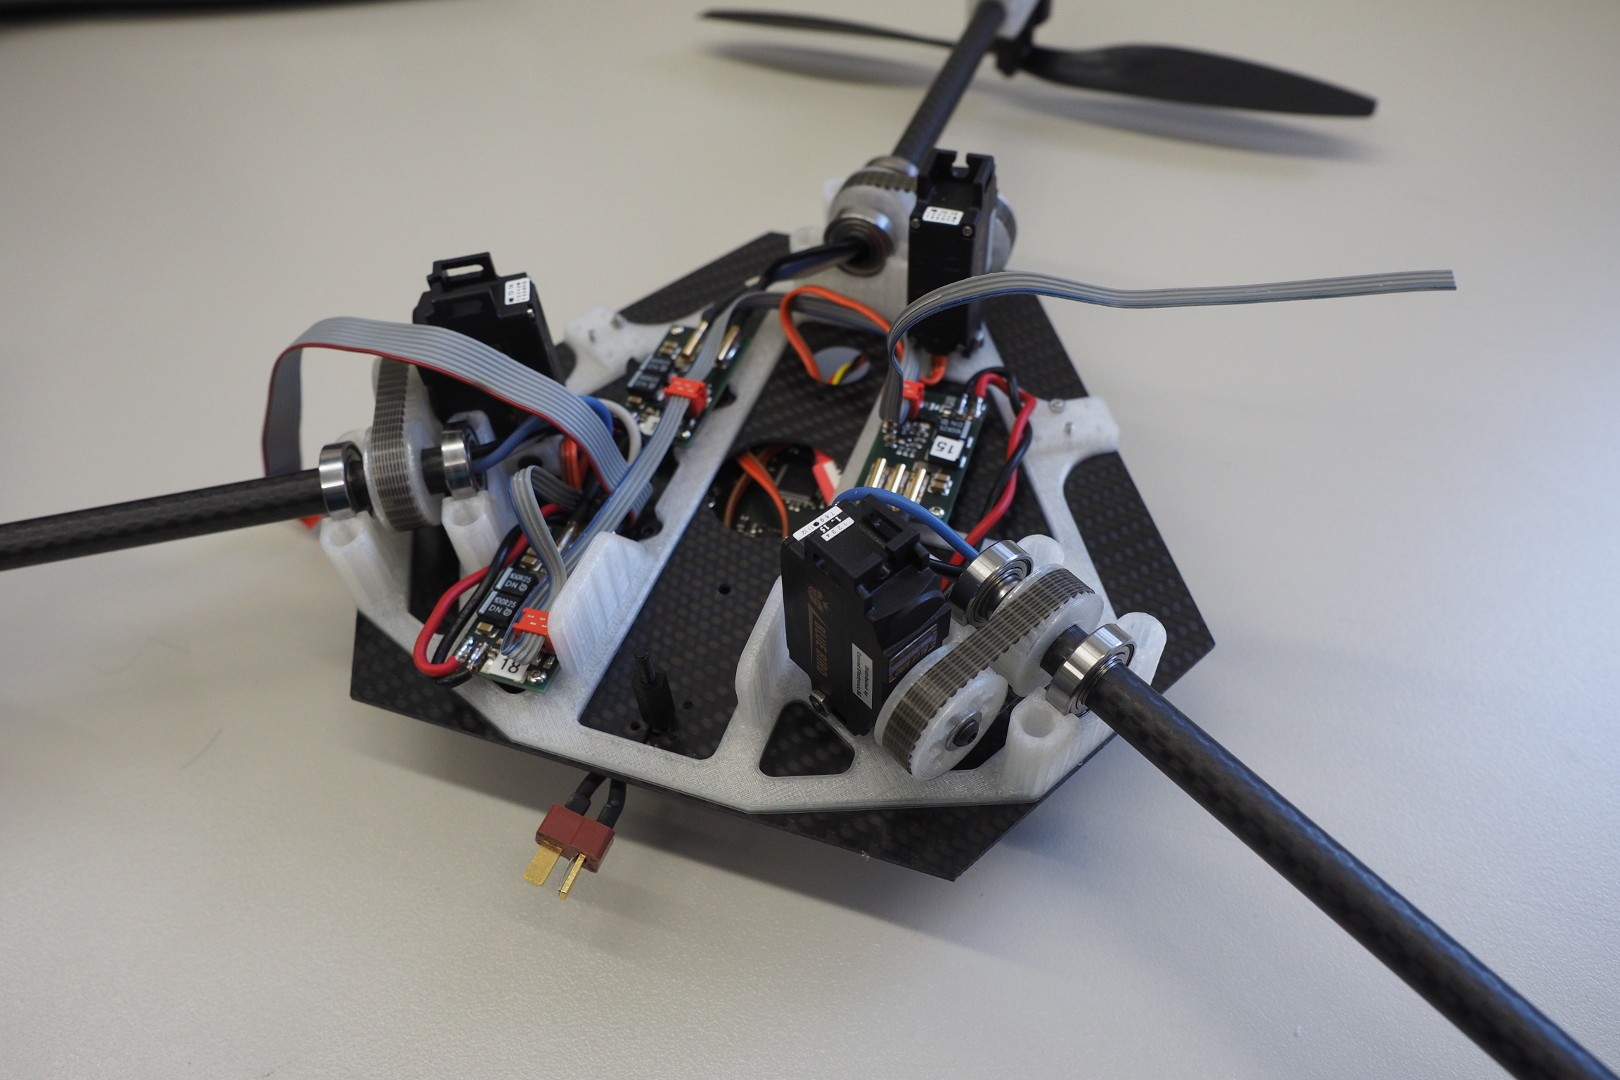
\includegraphics[height=6cm]{TriInnereien.jpg}
 \caption{Disassembled central body of the LSR-tricopter}
 \label{fig:TriInnereien}
\end{figure}

\paragraph{Mechanical frame.}
The mechanical design of the LSR-quat and tricopter (see \autoref{fig:LSRQuadAndTri}) is kept as simple as possible.
A central body holds the electronic parts including the battery.
It is a sandwich of two waterjet cutted carbon fiber plates that clamp together the internal 3d printed parts. 
These in turn clamp the carbon fiber tubes, the arms, or in the case of the tricopter its bearings, see \autoref{fig:TriInnereien}.
From there, carbon fiber tubes (the arms) stretch out to hold the propeller motors.
The propellers are directly bolted to their motors.
The radius at which the propellers are attached is intenionally the same for quad and tricopter, $\ArmRadius = 240\,\unit{mm}$.
The outer, flexible carbon-fiber rings serve as collision protection and landing skid.

\paragraph{Propeller drive.}
Quad and Ticopter share the same $10'' = 254\,\unit{mm}$ propellers, brushless DC motors and driver electronics.
The driver electronics and firmware is also an LSR development but will not be discussed further in this work.
Overall the drive allows for angular velocities up to $120\,\unit{Hz}$, corresponding to a maximum thrust of about $8\,\unit{N}$.
More crucially, it allows for very fast response times including active braking by feeding current back into the battery.

For the tricopter, the tilting mechanism is driven by a hobbyist servo drive that is connected to a gear on the arm by a toothed-belt (see \autoref{fig:TriInnereien}) and allows for tilt angles of $\pm 75^\circ$.

\paragraph{Sensors.}
Quad and Ticopter utilize the same sensors:
An inertial measurement unit (IMU) VN100s from \textsc{VectorNav} is mounted on the central body to measure its angular velocity and inertial acceleration.
It also contains an internal algorithm for bias and attitude estimation which is used for outdoor experiments which are not subject of this work.

Inside the LSR lab, a camera-based motion capture system (MOCAP) from \textsc{Vicon} measures position and attitude by way of reflective markers on the multicopters.
The motion capturing software runs on the ground station Windows 7 PC and the measurements are transfered to the multicopter processor via wireless link.
Overall, this results in a low sampling rate and significant latency in these measurements.
The algorithm used to fuse the high bandwidth IMU measurements with the MOCAP measurements will be presented in the following section.

\paragraph{User interface.}
A \textsc{Futaba} two-joystick remote control with several additional analog and digital inputs is used as a reliable and near real-time user interface.
It is used for manual piloting the multicopters as well as realizing security mechanisms like triggering emergency landing or even propeller shutdown.

The ground station computer runs a graphical user interface (GUI) implemented in \textsc{Matlab}. 
It displays and may record realtime data and can issue discrete commands to the multicopter controller.
Furthermore, this software also handles the forwarding of the MOCAP data. 
The communication link is realized by two XBee S6B Wi-Fi modules.

\paragraph{Mainboard \& processor.}
The center of the onboard electronics is a custom build mainboard.
It transforms and distributes the battery power to the other components and connects the data lines of the sensors and actuators to the main processor:
An Atmel AT32UC3C 32-bit, 66~\unit{MHz} microcontroller with FPU.

Overall, the relevant hardware components of the LSR-Multicopters are illustrated in \autoref{fig:MulticopterRealizationOverview}.


\begin{figure}[p]
 \centering
 \footnotesize
 \newcommand{\macGroundstation}{\textcolor{white}{\textbf{Groundstation} (Win7 PC)}}
 \newcommand{\macMulticopterRealization}{\textcolor{white}{\textbf{Multicopter}}}
 \newcommand{\macRBSI}{\textcolor{white}{\textbf{rigid}}}
 \newcommand{\macRBSII}{\textcolor{white}{\textbf{body}}}
 \newcommand{\macRBSIII}{\textcolor{white}{\textbf{system}}}
 \newcommand{\macMCI}{\textcolor{white}{\textbf{main}}}
 \newcommand{\macMCII}{\textcolor{white}{\textbf{controller}}}
 \input{graphics/MulticopterRealizationOverview.pdf_tex}
 \caption{Multicopter Hardware realization}
 \label{fig:MulticopterRealizationOverview}
%\end{figure}
\vspace{5mm}
 \input{graphics/MicocontrollerCodeStructure.pdf_tex}
 \caption{Controller code structure}
 \label{fig:MicocontrollerCodeStructure}
%\begin{figure}[hb]
\vspace{5mm}
 \footnotesize
 \input{graphics/StructureMulticopterAgent.pdf_tex}
 \caption{Structure of the Multicopter Agent}
 \label{fig:StructureMulticopterAgent}
\end{figure}


\paragraph{Firmware.}
The firmware on the main processor does not utilize an operation system but is programmed directly using C \& C++ code compiled by the \texttt{avr32-gcc}.
It uses the Atmel software framework as low level interface to the microcontroller peripherals.
On the top level, the template library \textsc{Eigen} offeres linear algebra objects and routines for the rigid body controller.
A rough overview of the microcontroller firmware is given in \autoref{fig:MicocontrollerCodeStructure}.

\paragraph{Multicopter agent.}
The critical control part of the multicopter firmware, here called \textit{multicopter agent}, is also used in a \textsc{Simulink} simulation of the closed loop with a multicopter model.
To be precise, the same cpp files are included in the either the firmware compilation as in the compilation of the simulink block. 

The multicopter model, the estimation of its parameters and experimental validation will be discussed in the next section.
For this work, the feedback controller for quad and tricopter are of paramount interest.
However, for its realization we need an accurate state estimation, the realization of the control forces and a reasonable reference generation.
These are also parts of the multicopter agent, as illustrated in \autoref{fig:StructureMulticopterAgent} and will be subject of ne next sections.